Ein ungesättigter Dampf steht nicht im Gleichgewicht mit seiner Flüssigkeit: Sein Druck ist kleiner als der Sättigungsdampfdruck bei derselben Temperatur. Er verhält sich näherungsweise wie ein ideales Gas, und sein Druck hängt (anders als beim gesättigten Dampf) nicht nur von der Temperatur ab, sondern auch von der Dampfmenge und vom Volumen. Eine eindeutige Dampfdruckkurve gibt es deshalb nicht.

Erwärmt man eine bestimmte Menge ungesättigten Dampfs in einem geschlossenen Gefäss (Volumen konstant), so ist der Druck proportional zur absoluten Temperatur: Im $p(T)$-Diagramm ist das eine \textbf{Gerade, deren Verlängerung durch den absoluten Nullpunkt geht} (rot). Sie liegt unterhalb der Dampfdruckkurve des gesättigten Dampfes (blau) und steigt viel weniger steil an als diese.

\begin{center}
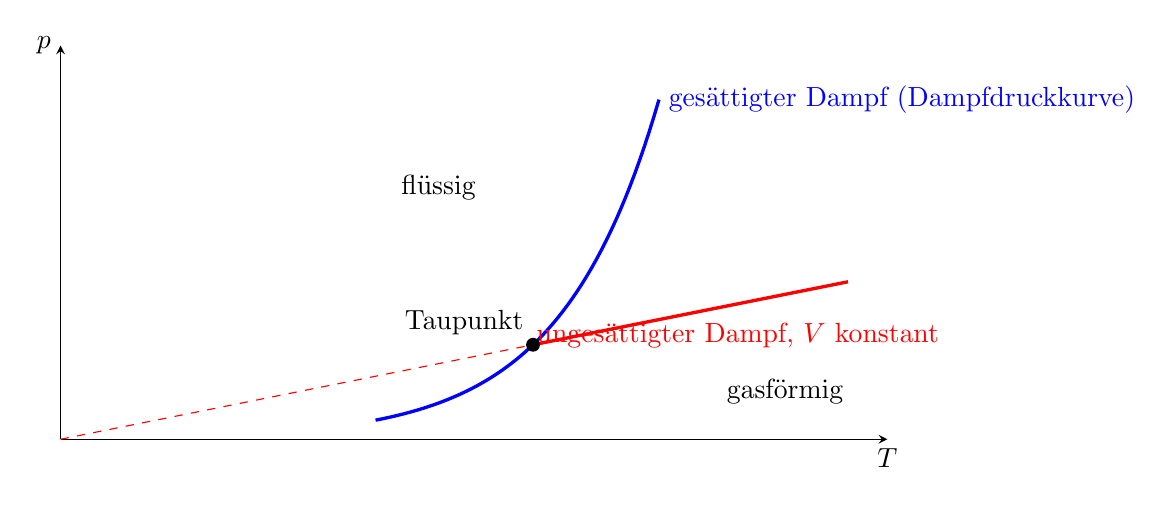
\begin{tikzpicture}[>=stealth]
 \draw[->] (0,0) -- (10.5,0) node[below] {$T$};
 \draw[->] (0,0) -- (0,5) node[left] {$p$};
 \draw[very thick, blue, domain=4:7.6, samples=60] plot (\x, {1.2*exp(0.8*(\x-6))});
 \node[blue, right] at (7.6,4.32) {gesättigter Dampf (Dampfdruckkurve)};
 \draw[dashed, red] (0,0) -- (6,1.2);
 \draw[very thick, red] (6,1.2) -- (10,2);
 \node[red, below] at (8.6,1.6) {ungesättigter Dampf, $V$ konstant};
 \fill (6,1.2) circle (2.5pt);
 \node[above left] at (6,1.2) {Taupunkt};
 \node at (4.8,3.2) {flüssig};
 \node at (9.2,0.6) {gasförmig};
\end{tikzpicture}
\end{center}

Kühlt man den Dampf ab, erreicht er beim Taupunkt die Dampfdruckkurve und ist gesättigt. Bei weiterem Abkühlen kondensiert ein Teil des Dampfes, und der Druck folgt der Dampfdruckkurve.
